\documentclass[times, utf8, seminar, numeric]{fer}
\usepackage{booktabs}
\usepackage{url}
\usepackage{indentfirst}
\usepackage{fancyvrb}
\usepackage{clrscode3e}
\usepackage{float}

\floatstyle{plain}
\newfloat{datoteka}{h}{lop}[chapter]
\floatname{datoteka}{Primjer}

\begin{document}

% Ukljuci literaturu u seminar
\nocite{*}

\title{Genetski algoritam primijenjen na funkcijsku aproksimaciju}

\author{Luka Mesarić}

\voditelj{doc. dr. sc. Marko Čupić}

\maketitle

\tableofcontents

\chapter{Uvod}

U ovom radu cilj je analiza primjene genetskog algoritma na pretragu beskonačnog skupa matematičkih funkcija unaprijed poznatog oblika.
Traži se funkcija jedne varijable u svrhu najbolje aproksimacije zadanog skupa podataka.
Implementiran je algoritam za pronalazak najprikladnije funkcije.

U svrhu razumijevanja genetskog algoritma, rad započinje definiranjem i objašnjavanjem osnovnih pojmova, nakon čega se razmatra pristup pri rješavanju konkretnog problema funkcijske aproksimacije.
U drugom dijelu rada opisane su mogućnosti izrađenog programa te se diskutira kvaliteta dobivenih rezultata.

Utvrđuje se da je algoritam odlično primjenjiv na dotičan problem.


\chapter{Genetski algoritam}

\section{Heuristički algoritmi}

\textit{Heuristički algoritmi} (\textit{heuristike}) tehnike su kojima se pronalaze približna rješenja problema čije bi egzaktno rješavanje iziskivalo previše vremena ili koje uopće nije moguće egzaktno riješiti~\cite{Cupic}.
Žrtvujući preciznost ili optimalnost konačnog rezultata, heuristike probleme rješavaju znatno brže od drugih uobičajenih metoda, često u polinomijalnoj složenosti~\cite{WikiHeuristic}.\\

\textit{Metaheuristike} skupovi su algoritamskih koncepata kojima se traže, stvaraju ili odabiru druge heuristike s ciljem pronalaska dovoljno dobrog rješenja optimizacijskog problema~\cite{WikiMetaheuristic}.
Prema tome, metaheuristike su zapravo heuristike opće namjene~\cite{Cupic}.
One uzimaju uzorke iz skupa rješenja koji je prevelik za cjelovitu obradu.
Ne garantiraju da će konačno rješenje problema ujedno biti i globalno optimalno (globalni minimum).

\section{Evolucijski algoritmi}

\textit{Evolucijski algoritmi} (EA) metaheuristike su inspirirane Darwinovom teorijom evolucije~\cite{WikiEvolutionary}.
Pripadaju populacijskim algoritmima.
Evolucijski algoritmi rade s populacijom rješenja nad kojima primjenjuju evolucijske operatore (selekcija, križanje, mutacija, rekombinacija) čime populacija svakom generacijom postaje sve bolja~\cite{Cupic}.

Najbitnije pretpostavke koje se koriste, a koje proizlaze iz Darwinove teorije, su sljedeće:
\begin{itemize}
	\item plodnost vrsta: broj potomaka uvijek je veći nego što je nužno potrebno,
	\vspace{-1mm}
	\item broj jedinki u populaciji približno je konstantan,
	\vspace{-1mm}
	\item u populaciji nema identičnih jedinki,
	\vspace{-1mm}
	\item najveći dio varijacija prenosi se nasljeđivanjem.
\end{itemize}

\section{Genetski algoritam}

\textit{Genetski algoritam} (GA) jedna je od najpopularnijih metaheuristika iz skupine evolucijskih algoritama~\cite{WikiEvolutionary}.

Algoritam radi nad populacijom potencijalnih rješenja (engl. \textit{candidate solutions}), koja se još nazivaju i \textit{jedinkama} (engl. \textit{individuals}).
Svaka jedinka u populaciji ima skup svojstava koja ju određuju, a koja se nazivaju \textit{kromosomima}~\cite{WikiGenetic}.
Kromosom se sastoji od \textit{gena} (engl. \textit{genes}), svaki od kojih kodira jedan atribut jedinke.
Vrijednosti gena nazivaju se \textit{alelima} (engl. \textit{alleles})~\cite{Kuthan2007GeneticAI}.
Geni, a posljedično i kromosomi, ono su što se mijenja evolucijom i što određuje \textit{dobrotu} (engl. \textit{fitness}) jedinke.

\textit{Dobrota} označava u kojoj mjeri neka jedinka zadovoljava svojstva traženog rješenja, a predstavljena je realnim brojem bez mjerne jedinice.
Što je dobrota jedinke veća, to je ona bliža ispravnom rješenju. 
Jedinke s malom dobrotom daleko su od traženog rješenja i imaju manju vjerojatnost biti odabrane za sljedeću iteraciju u evoluciji.\medskip

Za provođenje GA potrebno je odrediti dva modela:
\begin{itemize}
	\item funkciju dobrote
	\vspace{-1mm}
	\item reprezentaciju genoma (kromosoma).
\end{itemize}
\medskip

\textit{Funkcija dobrote} (engl. \textit{fitness function}) koristi se za izračun dobrote pojedine jedinke, tj. kromosoma.
Njeno modeliranje često predstavlja veliki izazov u primjeni GA pri rješavanju stvarnih problema~\cite{WikiFitness}.
Naime, tijekom brojnih iteracija GA funkcija dobrote evaluira se za svaku jedinku, što lako može rezultirati stotinama milijuna izračuna.
Ako se evaluacija ne izvršava brzo, cijeli algoritam može biti usporen do mjere u kojoj više nije upotrebljiv.
Iz tog, kao i iz drugih sličnih razloga, ponekad je nužno pribjeći aproksimativnim izračunima.
Primjeri su modeli koji poznaju dobrotu nekog konačnog skupa uzoraka, a ostale vrijednosti računaju interpolacijom, regresijom ili pak umjetnim neuronskim mrežama~\cite{WikiFitnessApprox}.

\textit{Reprezentacija genoma} (engl. \textit{genetic representation}) način je prikaza i pohrane kromosoma~\cite{WikiGeneRepres}.
Najčešći načini zapisivanja su \textit{prikaz nizom bitova} (engl. \textit{binary encoding}), \textit{prikaz poljem ili vektorom brojeva} (engl. \textit{value encoding}), \textit{prikaz permutacijama i matricama} (engl. \textit{permutation encoding}) te \textit{prikaz stablima} (engl. \textit{tree encoding})~\cite{Kuthan2007GeneticAI}~\cite{Cupic}.
Kao i u slučaju funkcije dobrote, ovo modeliranje može uzrokovati velike poteškoće u primjeni GA na komplicirane probleme.
Razlog je zato što zapis kromosoma mora biti pogodan za smisleno korištenje evolucijskih operatora križanja i mutacije.

Kako bi se u svakoj generaciji populacija mogla poboljšavati, potrebni su evolucijski operatori selekcije, križanja i mutacije~\cite{Cupic}.

Operatorom \textit{selekcije} (engl. \textit{selection}) osigurava se mehanizam diferencijacije rješenja prema njihovoj kvaliteti.
Cilj je kvalitetnijim rješenjima pružiti mogućnost generiranja novih rješenja, odnosno jedinke koje ne predstavljaju kvalitetna rješanja isključiti iz procesa reprodukcije. 
Primjeri selekcija su turnirske selekcije, selekcija linearnim rangiranjem i proporcionalna selekcija~\cite{Cupic}.

Operatorom \textit{križanja} (engl. \textit{crossover}) jedinke razmjenjuju gene.
Iz dvije se jedinke \textit{roditelja} stvara jedna nova jedinka \textit{dijete}.
Ideja odabira dva roditelja proizlazi iz najčešćeg načina razmnožavanja u prirodi.
Međutim, toga se nije nužno pridržavati te je dopušteno koristiti i više od dvaju roditelja za stvanje jednog djeteta.
Postoji iznimno velik broj postupaka kojima se može obavljati križanje.
Ključnu ulogu ima reprezentacija genoma.
Jednostavna su križanja s jednom ili više točaka prekida.
U slučaju prikaza poljem brojeva, križanja se svode na razne aritmetičke operacije.

Operatorom \textit{mutiranja} (engl. \textit{mutation}) mijenja se vrijednost jednog ili više slučajno odabranih gena u kromosomu jedinke.
Mutiranjem se proširuje genetska raznolikost populacije na način na koji to nije moguće napraviti samo križanjem.
Optimalna vjerojatnost mutacije u velikoj mjeri ovisi o konkretnom problemu koji se rješava.
Ipak, ako se vjerojatnost mutacije postavi na preveliku vrijednost, učinak će vrlo vjerojatno biti negativan.
Zbog konstantnih mutacija često će biti onemogućena konvergencija k ispravnom rješenju jer će u svakoj generaciji populacija biti preplavljena slučajno generiranim jedinkama.

Pseudokod genetskog algoritma prikazan je u nastavku. Pseudokod je preuzet iz izvora~\cite{GaPseudocode}.
\begin{codebox}
	\Procname{$\proc{Genetic algorithm pseudocode}$}
	\li $\id{t} = 0;$
	\li $initialize(P(t=0));$
	\li $evaluate(P(t=0));$
	\li \While $isNotTerminated()$ \Do
	\li $P_p(t) = P(t).select Parents();$
	\li $P_c(t) = reproduction(P_p);$
	\li $mutate(P_c(t));$
	\li $evaluate(P_c(t));$
	\li $P(t+1) = buildNextGenerationFrom(P_c(t), P(t));$
	\li $t=t+1;$
	\End
\end{codebox}


\chapter{Teorijski pristup primjeni algoritma}

Razmotrimo problem određivanja realne funkcije jedne realne varijable $f(x)$ koja najbolje opisuje ulazne podatke $P$.
Podatci su predstavljeni skupom od $n \in \mathbb{N}$ točaka u Kartezijevom koordinatnom sustavu:
\begin{equation}
	P = \{(x_i, y_i) \in \mathbb{R} \times \mathbb{R}\ \ |\ \ i = 1, \dots, n\} \label{eq:P}
\end{equation}

Za svaki ulazni skup točaka može se pronaći beskonačno mnogo funkcija koje ga opisuju.
Stoga je potrebno postaviti neka ograničenja.
Konkretno, zahtijeva se da oblik funkcije $f$ unaprijed bude poznat, dok će (neki) realni koeficijenti biti varijabilni.
Ako u funkciji postoji $k \in \mathbb{N}$ koeficijenata, oni će biti opisani vektorom $\vec{Z} \in \mathbb{R}^k$.

Definirajmo realnu funkciju $g(x, \vec{Z})$ koja upravo predstavlja poopćenje funkcije $f(x)$ na način da definira mjesta za koeficijente, a fiksira poznati dio funkcije.

Kvantificiranje koliko dobro neka funkcija $g(x,\vec{Z_0})$ opisuje ulazne podatke $P$ provodit će se koristeći formulu za \textit{sumu kvadrata odstupanja} (engl. \textit{residual sum of squares})~\cite{WikiResidualSum}:
\begin{equation}
RSS(\vec{Z}) = \sum_{i=1}^{n}\left(y_i - g(x_i, \vec{Z})\right)^2\label{eq:RSS}
\end{equation}
U formuli \eqref{eq:RSS} oznake $x_i$ i $y_i$ predstavljaju vrijednosti $x$ i $y$-koordinata $i$-te točke iz ulaznih podataka $P$.
Zbog toga što je $\vec{Z_0} \in \mathbb{R}^k$ neki konkretan vektor, $g(x,\vec{Z_0})$ je funkcija jedne varijable.
Slično vrijedi i za izraz $g(x_i, \vec{Z})$ iz formule \eqref{eq:RSS}, jer je $\vec{Z}$ zapravo fiksiran kroz argument funkcije $RSS$.\\

Kako bi pri rješavanju problema bilo moguće primijeniti genetski algoritam, potrebno je odrediti reprezentaciju genoma, funkciju dobrote i genetske operatore.

S obzirom na to da se traži niz realnih koeficijenata $\vec{Z}$, prikaz poljem brojeva (engl.~\textit{value encoding}) nameće se kao najprikladnija reprezentacija genoma.
U tom slučaju geni predstavljaju pojedine koeficijente, dok su aleli vrijednosti tih koeficijenata.
Radi jednostavnost, jedinku ćemo poistovjetiti s vektorom koeficijenata te ćemo i nju označavati sa $\vec{Z}$.
Primijetimo da same jedinke nisu direktno povezane s traženom matematičkom funkcijom, već pohranjuju \textit{neke realne brojeve}.
Značenje tih brojeva, tj. alela, ponajprije interpretira funkcija dobrote.

Zbog toga što se genetskim algoritmom traže (lokalni) maksimumi, jedinkama za koje smatramo da su bliže ispravnom rješenju potrebno je pridijeliti veću dobrotu.
S druge strane, funkcija $RSS$ definirana formulom \eqref{eq:RSS} davat će manje vrijednosti za jedinke $\vec{Z}$ koje bolje opisuju podatke $P$, i te će vrijednosti uvijek biti nenegativne.
Prema tome, dva moguća jednostavna modela funkcije dobrote su negativna vrijednost i recipročna vrijednost funkcije $RSS$:
\begin{align}
fitness_1(\vec{Z}) &= -RSS(\vec{Z}) \label{eq:fitnessNeg}\\
fitness_2(\vec{Z}) &= \frac{1}{RSS(\vec{Z})} \label{eq:fitnessInv}
\end{align}
Funkcija $fitness_1$ za svaki će $\vec{Z}$ vraćati negativne vrijednosti, dok će funkcija $fitness_2$ vraćati samo pozitivne vrijednosti.
U oba slučaja kvalitetnijim jedinkama bit će pridružena veća vrijednost dobrote.

Realizacija operatora selekcije ne mora biti komplicirana.
U ovom slučaju dovoljna je standardna $3$-turnirska selekcija.

Zbog toga što se za reprezentaciju genoma koristi prikaz poljem realnih brojeva, za implementaciju operatora križanja najprikladnije je odabrati aritmetičko križanje, $BLX-\alpha$ križanje, prošireno komponentno križanje, ili neko njima slično.

Kod operatora mutiranja nema smisla odabrati verzije koje mijenjaju poredak gena.
Naime, već i susjedni geni mogu predstavljati koeficijente na sasvim različitim mjestima i sa sasvim različitim utjecajima na vrijednosti funkcije. 
Na primjer, zamjenom koeficijenata uz kubni i linearni član polinoma vrlo se vjerojatno neće dobiti kvalitetna jedinka.
U ovom je slučaju mutiranje prikladno implementirati kao malu promjenu vrijednosti nekog gena u kromosomu.


\chapter{Programska implementacija}

Svi programski kodovi javno su dostupni na \textit{GitHub} repozitoriju:\\
\url{https://github.com/LMesaric/Seminar-FER-2019}

Kako bi se program mogao izvoditi, na računalu je potrebno imati instalirane sve biblioteke navedene u nastavku.

Programska implementacija pridržava se svih ideja i principa razmatranih u prethodnom poglavlju.

Za implementaciju je korišten programski jezik \textit{Python}.
Od javno dostupnih i gotovih biblioteka, korištene su sljedeće:
\begin{itemize}
	\item \textit{DEAP Framework (Distributed Evolutionary Algorithms in Python)}~\cite{Deap} --- za obavljanje genetskih operacija križanja i mutacije te za selekciju,
	\item \textit{Matplotlib}~\cite{Matplotlib} --- za crtanja grafa funkcije koja je dobivena kao rješenje,
	\item \textit{NumPy}~\cite{Numpy} --- za ubrzanje provođenja računskih operacija,
	\item \textit{SymPy}~\cite{Sympy} --- za parsiranje korisničkog unosa (simbolički račun).
\end{itemize}
\bigskip

Prilikom pokretanja program od korisnika traži da kroz konzolu unese podatke: 
\begin{enumerate}
	\item relativan ili apsolutan put do datoteke s podatcima za aproksimaciju,
	\vspace{-2mm}
	\item tekstualnu reprezentaciju traženog oblika funkcije,
	\vspace{-2mm}
	\item maksimalan broj iteracija (generacija) prije zaustavljanja provođenja algoritma.
\end{enumerate}

U datoteci s podatcima u svakoj nepraznoj liniji mora biti zapisan jedan par $x$ i $y$ koordinata, razvojenih jednim ili više razmaka ili tabulatora.
Linije koje započinju znakovima "$//$" tretiraju se kao komentari i ignoriraju se.
Ako su podatci u datoteci generirani nekom poznatom (originalnom) funkcijom bez varijabilnih koeficijenata, ona se također može zapisati u datoteku.
Takva linija mora započeti znakom "$\#$".
Zapisana funkcija ni na koji način ne utječe na izvođenje algoritma ni na konačan rezultat, već samo služi kao kontrolni mehanizam za provjeru kvalitete rješenja.

\begin{datoteka}
	\begin{Verbatim}[fontsize=\small]
	# 0.4*sin(1.3*x-2.1)*exp(0.3*x-0.2)
	// sine and exponential, wide interval
	-10.00000	-0.009313
	-9.000000	-0.020770
	-8.000000	+0.001970
	-7.000000	+0.039268
	-6.000000	+0.024768
	-5.000000	-0.053665
	-4.000000	-0.083886
	-3.000000	+0.037204
	-2.000000	+0.179718
	-1.000000	+0.061997
	+0.000000	-0.282694
	+1.000000	-0.317120
	+2.000000	+0.286088
	+3.000000	+0.784435
	+4.000000	+0.045211
	+5.000000	-1.396684
	+6.000000	-1.091025
	+7.000000	+1.757017
	\end{Verbatim}
	\caption[Sadržaj datoteke s podatcima]
	{\label{PrimjerDatoteke}Primjer datoteke s podatcima koja sadrži komentare i originalnu funkciju.}
\end{datoteka}

Funkcija koju korisnik zadaje kroz konzolu sadržava nepoznate koeficijente.
Preporuča se te koeficijente označiti velikim slovima, poput $A, B, C, \dots$, iako su moguće i druge oznake.
Slova $E$ i $I$ su izuzetak -- ona će se interpretirati kao Eulerov broj, odnosno imaginarna jedinica.
Primjeri dopuštenih unosa slijede u nastavku.
\begin{align}
	&\texttt{A*x\textasciicircum 3+B*x\textasciicircum 2+C*x+D} \label{ex:1}\\
	&\texttt{A+B*sin(C*x+D)} \label{ex:2}\\
	&\texttt{A*sin(B*x+C)*exp(D*x+F)} \label{ex:3}\\
	&\texttt{A+B*sqrt(abs(C*x+D))} \label{ex:4}\\
	&\texttt{sqrt(abs(x))} \label{ex:5}\\
	&\texttt{AH*sin(BU*x+CR)*exp(D*x+F)} \label{ex:6}
\end{align}

Primjer \ref{ex:5} pokazuje da unos uopće ne mora imati slobodnih koeficijenata, dok primjer \ref{ex:6} pokazuje da se pojedini koeficijenti mogu označiti i nizom znakova.
Primjer \ref{ex:6} ekvivalentan je primjeru \ref{ex:3}.

Od mogućih implementacija operatora selekcije, $3$-turnirska selekcija pokazala je najbolje rezultate.

Za operator križanja odabrana je mješavina aritmetičkog križanja i proširenog komponentnog križanja~\cite{Cupic}.
\textit{DEAP} takvo križanje obavlja \texttt{cxBlend} funkcijom.
Uočeno je da se najbolji rezultati dobivaju za koeficijent $\alpha = 0.20$, odnosno kada je $\lambda \in \left[ -0.20, 1.20 \right]$.
Parametar $\lambda$ slučajno se odabire za svaki gen u kromosomu.

Za operator mutiranja korištena je Gaussova mutacija~\cite{WikiMutation}, odnosno \texttt{mutGaussian} funkcija.
Ako je jedinka odabrana za mutiranje, neki se njezini koeficijenti uvećavaju ili umanjuju za slučajnu vrijednost dobivenu iz Gaussove distribucije.
Najbolji rezultati dobiveni su za $\mu = 0$ i $\sigma = 0.15$, uz vjerojatnost mutacije postavljenu na $0.4$.
Uz razne veće i manje vrijednosti parametra $\sigma$ također se mogu dobiti kvalitetni rezultati.
Bitno je napomenuti da se uz veće vjerojatnosti mutiranja redovito dobivaju bolji rezultati.
Razlog tome je što je selekcija implementirana na način da se kvalitetne jedinke kloniraju, a nekvalitetne se eliminiraju.
Klonovi ne pridonose raznolikosti populacije pa ih je potrebno mutirati, što je jednostavno ostvarivo povećanjem vjerojatnosti mutiranja.
Dodatno, učestalije mutacije pomažu da populacija prerano ne zapne u krivom lokalnom maksimumu.
Uz veliku vjerojatnost mutacije populacija rijetko konvergira.

Za funkciju dobrote odabrana je implementacija bazirana na jednadžbi \eqref{eq:fitnessNeg}, dakle negativna vrijednost sume kvadrata odstupanja.
Razlog takve odluke jest svojstvo \textit{DEAP Frameworka} koje omogućava dodavanje težinskog faktora izračunatoj dobroti.
\textit{DEAP} uvijek traži jedinke s najvećom dobrotom pa se postavljanjem težine na vrijednost $-1.0$ vrlo jednostavno dobiva efekt traženja minimalne vrijednosti dobrote.
Dodatno, tada se dobrota računa samo kao $RSS$, bez ikakvih izmjena, čime ujedno predstavlja i grešku aproksimacije.
Radi potpunosti, testirana je i implementacija bazirana na formuli \eqref{eq:fitnessInv} te su postignuti vrlo slični rezultati.\\

U najgorem slučaju izvođenje programa zaustavlja se u trenutku kada je dosegnut maksimalno dozvoljen broj iteracija.
Otprilike $200$ generacija dovoljno je za kvalitetnu aproksimaciju većine funkcija.
Ako se u manjem broju generacija pronađe rješenje čija je pogreška aproksimacije manja od $10^{-7}$, program će se automatski zaustaviti.
Korisnik tijekom izvođenja programa može uočiti da nakon nekog trenutka više nema značajnog napretka u pronalasku boljeg rješenja.
Ako ne želi čekati da se provede maksimalan broj iteracija, program je moguće prijevremeno zaustaviti pritiskom \texttt{Ctrl+C} na tipkovnici.
Izvođenje neće biti nasilno prekinuto, već će uredno biti dovršene sve operacije nad trenutnom populacijom i nakon toga će biti prikazani rezultati kao i u slučaju kada program završi bez korisnikove intervencije.

Tijekom izvođenja programa za svaku se generaciju u konzolu ispisuje pogreška aproksimacije najbolje jedinke.
Po završetku izvođenja prikazuju se oznake i vrijednosti svakog koeficijenta najbolje jedinke posljednje populacije.
Dodatno, ispisuje se i konačan oblik funkcije dobivene aproksimacijom, kao i njezina apsolutna pogreška.
Uz ispis u konzolu prikazuje se i graf rješenja.

Crvene točke na grafu predstavljaju ulazne podatke.
Punom linijom nacrtana je funkcija dobivena genetskim algoritmom.
Njezina jednadžba napisana je odmah iznad grafa.
Ako je zapisana u datoteci, originalna funkcija bit će nacrtana točkastom linijom zelene boje.

Graf je moguće pomicati i uvećavati.
Inicijalno će koordinatni sustav biti upravo dovoljno velik kako bi mogli biti prikazani svi podatci i vrijednosti funckije.\\

U nastavku slijede primjeri rezultata izvođenja programa za ulazne podatke prikazane u primjeru \ref{PrimjerDatoteke}.
Tražena funkcija ima oblik \texttt{A*sin(B*x+C)*exp(D*x+F)}.
Maksimalan broj generacija postavljen je na $200$, dok je veličina populacije postavljena na $2000$ jedinki.

Na slici \ref{Graph_GoodFreq} prikazana je najbolja jedinka $200.$ iteracije, koja se u potpunosti preklapa s originalnom funkcijom.
Njezina pogreška aproksimacije iznosi $1.8\cdot 10^{-4}$.

\begin{figure}[h]
	\centering
	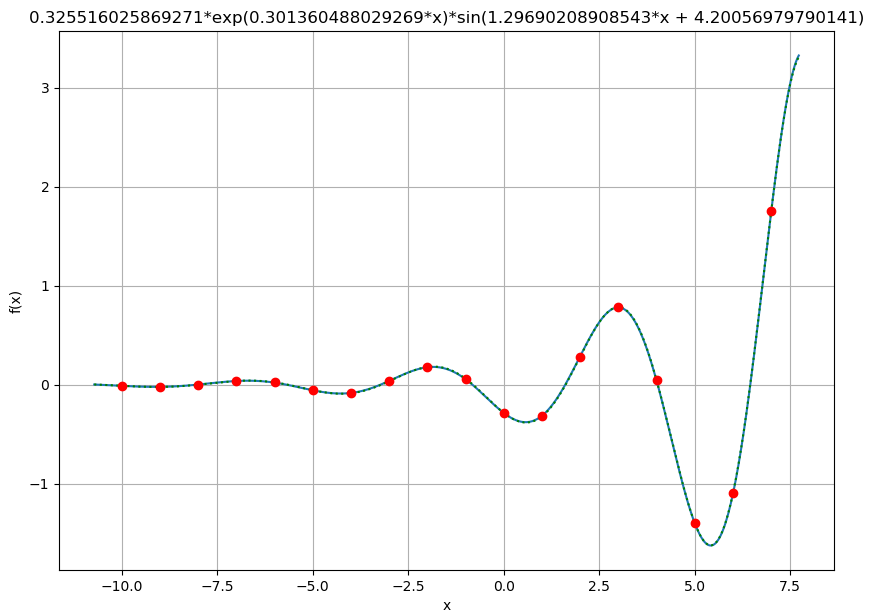
\includegraphics[width=1\textwidth]{figures/Graph_GoodFreq.png}
	\caption{\label{Graph_GoodFreq}Najbolja jedinka nakon $200$ iteracija, preklopljena s originalnom funkcijom.}
\end{figure}

Rijetko je kada originalna funkcija jedina funkcija kojom se podatci mogu aproksimirati.
Kada se koriste trigonometrijske funkcije, poput sinusne, nerijetko se događa da dobiveno rješenje ima višestruko veću frekvenciju od frekvencije originalne funkcije.
Primjer takvog rezultata prikazan je na slici \ref{Graph_HighFreq}.
Iako se dobivena funkcija ne može koristiti za interpoliranje podataka, njezina pogreška zapravo je vrlo mala: $4.1\cdot 10^{-4}$.

\begin{figure}[h]
	\centering
	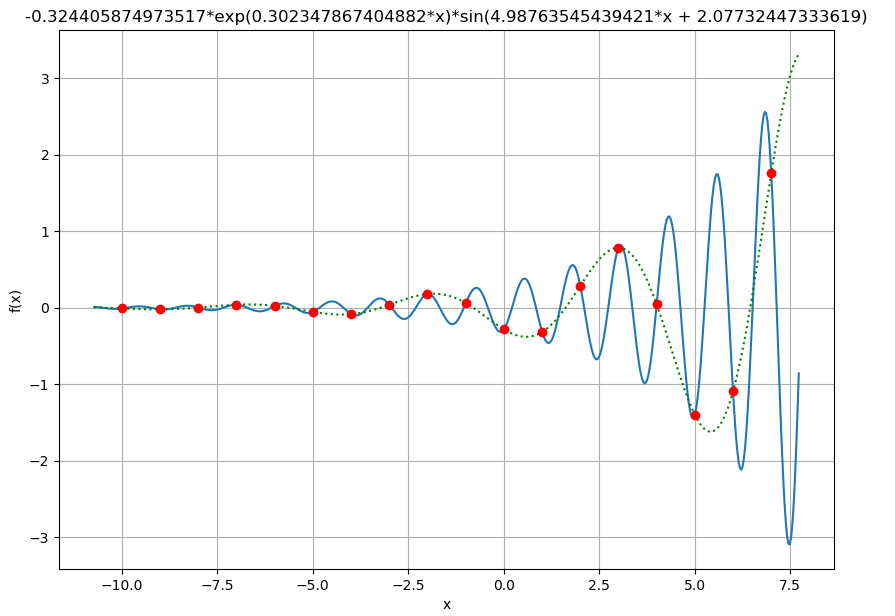
\includegraphics[width=1\textwidth]{figures/Graph_HighFreq.png}
	\caption{\label{Graph_HighFreq}Najbolja jedinka nakon $200$ iteracija, uz jasno vidljivu originalnu funkciju.}
\end{figure}

Na grafu prikazanom slikom \ref{Graph_2000} nacrtano je svih $2000$ jedinki nakon $200$ iteracija.
Jasno je uočljiva konvergencija populacije prema optimalnom rješenju.

\begin{figure}[h]
	\centering
	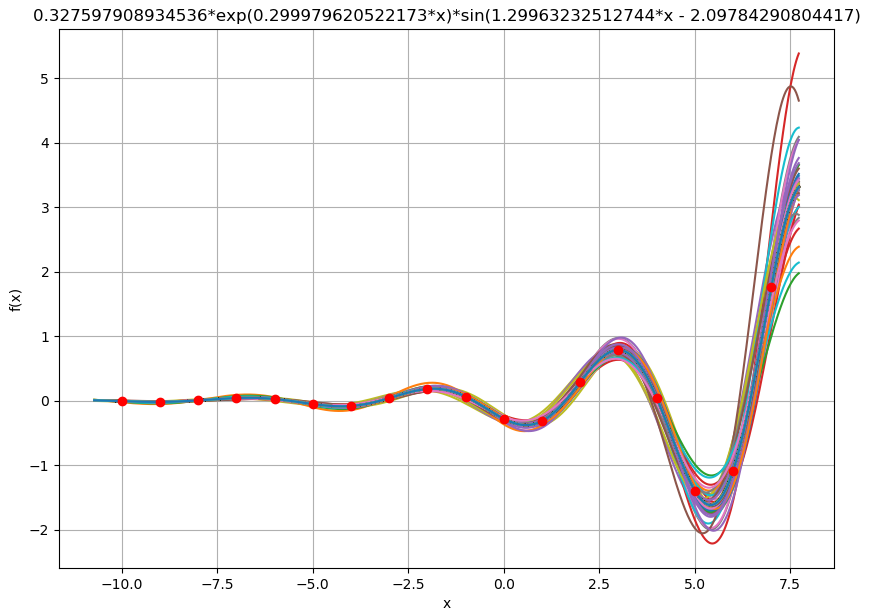
\includegraphics[width=1\textwidth]{figures/Graph_2000.png}
	\caption{\label{Graph_2000}Populacija od $2000$ jedinki nakon $200$ iteracija.}
\end{figure}

Posljednji primjer malo se razlikuje od ostalih.
Originalna funkcija u potpunosti je jednaka, ali se aproksimiraju podatci na manjem intervalu oko ishodišta.
Dodatno, traži se aproksimacija polinomom trećeg stupnja: \texttt{A*x\textasciicircum 3+B*x\textasciicircum 2+C*x+D}.
Rezultat takve aproksimacije prikazan je na slici \ref{Graph_Poly}.
Već se u približno $30.$ generaciji dobiva rješenje čija se pogreška aproksimacije, zaokružena na dvije značajne znamenke, više ne mijenja i iznosi $0.0071$.
Program je pokrenut dvadesetak puta i svako izvršavanje rezultiralo je takvim ponašanjem.
Zanimljivo je primijetiti da je dobivena funkcija upravo jednaka najboljem mogućem rješenju za polinom trećeg stupnja, što je potvrđeno kubnom regresijom.

\begin{figure}[h]
	\centering
	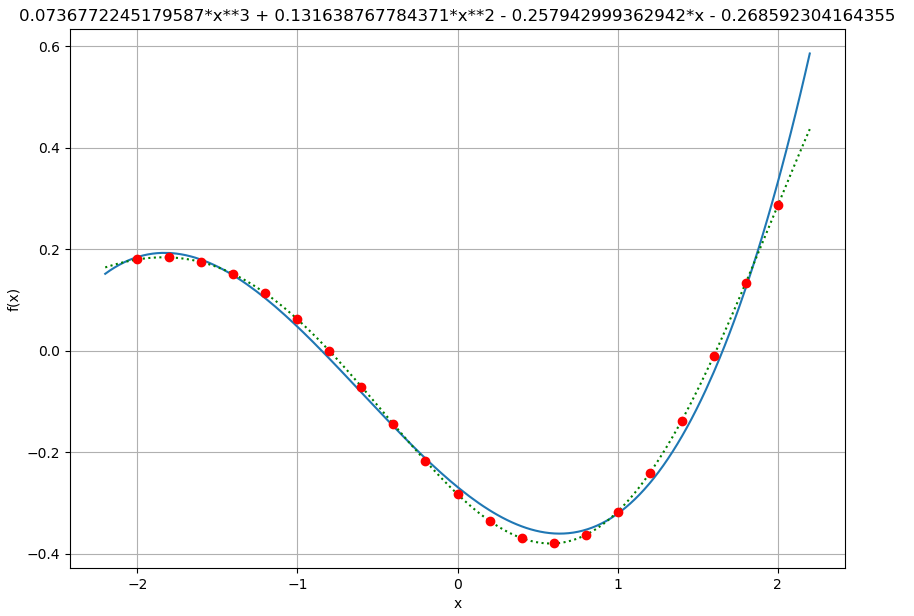
\includegraphics[width=1\textwidth]{figures/Graph_Poly.png}
	\caption{\label{Graph_Poly}Aproksimacija polinomom trećeg stupnja.}
\end{figure}


\chapter{Zaključak}

Genetski algoritam moguće je primijeniti pri rješavanju raznolikih problema, pa tako i tematiziranog problema funkcijske aproksimacije.
Izrađenim programom uspješno je dokazana upotrebljivost algoritma.


\bibliography{literatura}
\bibliographystyle{fer}


\chapter{Sažetak}

U ovom radu analizirana je primjena genetskog algoritma na pretragu beskonačnog skupa matematičkih funkcija unaprijed poznatog oblika.
Svrha je pronalazak funkcije jedne varijable koja najbolje aproksimira zadani skup ulaznih podataka.
Razmatranje je popraćeno konkretnom implementacijom algoritma za pronalazak najprikladnije funkcije te njezinim grafičkim prikazom.

Nakon pregleda osnovnih pojmova nužnih za razumijevanje genetskog algoritma slijedi teorijsko razmatranje načina njegove primjene na konkretan problem funkcijske aproksimacije.
U drugom dijelu rada opisane su mogućnosti izrađenog programa te se diskutira kvaliteta dobivenih rezultata.

Utvrđuje se da je algoritam odlično primjenjiv na dotičan problem.
\bigskip

Svi programski kodovi javno su dostupni na \textit{GitHub} repozitoriju:\\
\url{https://github.com/LMesaric/Seminar-FER-2019}


\end{document}
